\documentclass{beamer}
\usepackage[utf8]{inputenc}
\usepackage[T1]{fontenc}
%\usepackage[french]{babel}
\usepackage{amsmath, amsfonts, amsthm, amssymb}
\usepackage{hyperref}
\usepackage{tcolorbox}

% to make larger title
\setbeamertemplate{frametitle}{%
	\begin{beamercolorbox}[wd=\linewidth, ht=0.5cm, dp=0.2cm]{frametitle}
		\usebeamerfont{frametitle}\insertframetitle
	\end{beamercolorbox}
}

\beamertemplatenavigationsymbolsempty

\newcommand{\cmd}[1]{\fbox{\color{black}\texttt{#1}}}
\newtheorem{exo}{Exercise}

\title{GIT tutorial}
\author{Pauline Hubert and Nadia Lafrenière}
\date{FPSAC software days, July 2019}
\begin{document}
	\maketitle
	\begin{frame}{Motivations}
		\begin{figure}[h]
			\centering
			
\includegraphics[scale=.28]{phd101212s.png}
		\end{figure}
	\end{frame}

	\begin{frame}{What software to use? Pros and cons}
		\begin{tabular}{lp{0.35\linewidth}p{0.35\linewidth}}
%			\hline
			& Pros & Cons\\
			\hline
			Email & "Easy" to use & So many!\\
			\hline
			Overleaf & Many people can work at the same time & Only online, latex only\\
			\hline
			Dropbox & Easy to use & No two people can work at the same time, no version control\\
			\hline
			Git & Version control, automatic fusion of modifications, any file type & More difficult to start\\
%			\hline
		\end{tabular}
	\end{frame}

	\begin{frame}{What is Git?}
		Git is a \textit{version control software}. \newline
		
		\begin{itemize}
			\item It keeps track of every modifications.
			\item You can go back in time to a previous version.
			\item It allows many people to work in parallel.
		\end{itemize}	
	\end{frame}

	\begin{frame}{Online servers for Git}
		Store your data somewhere. \newline 
			\begin{itemize}
				\item Local: on your computer.
				\item Online servers: Github, Bitbucket, GitLab, your university server, etc. \newline
			\end{itemize}
		If you use an online server, you will also have a local version on your computer. If you want to work with other people, you have to use a server. 
	\end{frame}

	\begin{frame}{Now that you are convinced... Installation}
		\begin{itemize}
			\item Linux : Type in shell \texttt{sudo apt install git}
			\item MacOS : Go to \url{https://git-scm.com/download/mac}
			\item Windows : Go to \url{https://gitforwindows.org}
		\end{itemize}
	\end{frame}

	\begin{frame}[fragile]{Configuration \hfill \cmd{config}}
	To share code, you need to identify yourself:
	\begin{verbatim}
$ git config --global user.name "John Doe"
$ git config --global user.email "john.doe@email.com"
	\end{verbatim}
	Please, do not use this example as is, put your real name instead!
	\end{frame}

	\begin{frame}[fragile]{Getting code: cloning \hfill \cmd{clone}}
		To get code from a remote repository:
		\begin{verbatim}
		$ git clone https://address-of-the-repo.git
		\end{verbatim}
		Maybe some of you did, yesterday,
		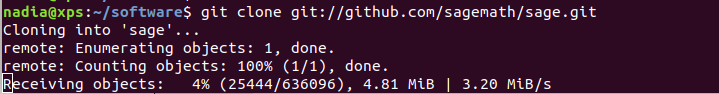
\includegraphics[width=\linewidth]{clone}
		\pause
		\begin{exo}
			Clone the repository containing this talk.
			\url{https://github.com/phubert/git_sagedays2019.git}
		\end{exo}
	\end{frame}

	\begin{frame}[fragile]{What's happening?\hfill \cmd{status}}
		Lost? You wanna check if everything went well? This command is your friend!
		\begin{verbatim}
$ git status
		\end{verbatim}
		\begin{center}
			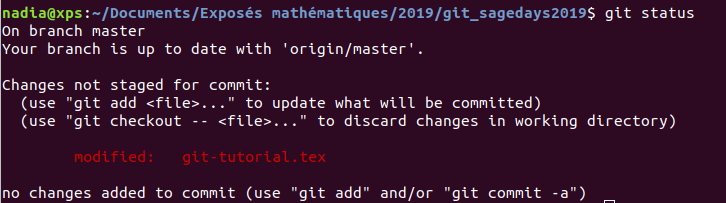
\includegraphics[width=\linewidth]{status}
		\end{center}
	\end{frame}

	\begin{frame}[fragile]{First steps: Starting to use Git on a project\hfill \cmd{init}}
		Two ways to start: 
		\begin{itemize}
			\item Use an existing local project.
			\item Create a new project on a server (e.g. \href{https://github.com/}{Github}) and clone it. \newline
		\end{itemize}
	
		If your already have a project.
		\begin{enumerate}
		\item  In the directory containing your files, run the command 
		\mbox{\texttt{git init}}.
		
		\item  (optional, recommended) Then, you can put your files on the server. For that, create a new \emph{empty} repository on the server and follow the instructions.
		
		The commands you will need are 
		\begin{verbatim}
			$ git remote add origin REPO_URL
			$ git push -u origin master
		\end{verbatim}
		
		\end{enumerate}   
	\end{frame}

	\begin{frame}[fragile]{Modifications \hfill \cmd{add}}
		Once you worked on your code/text, you will want to save the modifications. \newline
		
		To select the (new or modified) files that will be added to the modification use the command
		\begin{verbatim}
			$ git add FILE_NAME1 FILE_NAME2 ...
		\end{verbatim}
	\end{frame}

	\begin{frame}[fragile]{Modifications \hfill \cmd{commit}}	
		To save modifications, use the command \texttt{git commit}. \newline 
		
		Each time you make a commit, a text editor appears in your terminal and you have to write a short (but \textit{meaningful}) comment to describe your modifications. \newline
		
		If you modified only files that were already in the git repository you can also list the files directly in the commit command. 
		\begin{verbatim}
		$ git commit FILE_NAME1 FILE_NAME2 ...
		\end{verbatim}
		
		Two usefull options : \texttt{git commit -OPTS}, where \texttt{-OPTS} is
		
		\texttt{-a} allows you to save all the modified files with the same commit message.
		 
		\texttt{-m "Comment"} allows you to directly write your commit message in the command. 		
	\end{frame}

	\begin{frame}[fragile]{Sharing modifications \hfill \cmd{push}}
		For the moment, all your modifications are only saved in your local copy of your project. 
		
		After committing, you may want to share your modifications by adding them to the online repository. The command for that is 
		
		\begin{verbatim}
		$ git push
		\end{verbatim}
		
		You may be asked to enter your username and password at this point.
		
		You don't have to push every time you commit. You can push several commits at once, but your collaborators will not see the changes until you push. 
	\end{frame}
	
	\begin{frame}[fragile]{Getting updated code \& solving conflicts \hfill \cmd{pull}}
		To obtain the updated version of the project, use
		\begin{verbatim}
		$ git pull
		\end{verbatim}
		
		\textit{"What if one of my collaborator worked at the same time as me?"}
		
		If this happens, you will get an error message when you try to push. Then, read and follow the instructions!  
	\end{frame}

	\begin{frame}{Reviewing changes \hfill \cmd{diff}}
	You can look at what other people did:
	\begin{itemize}
		\only<1>{\item on a software\\
		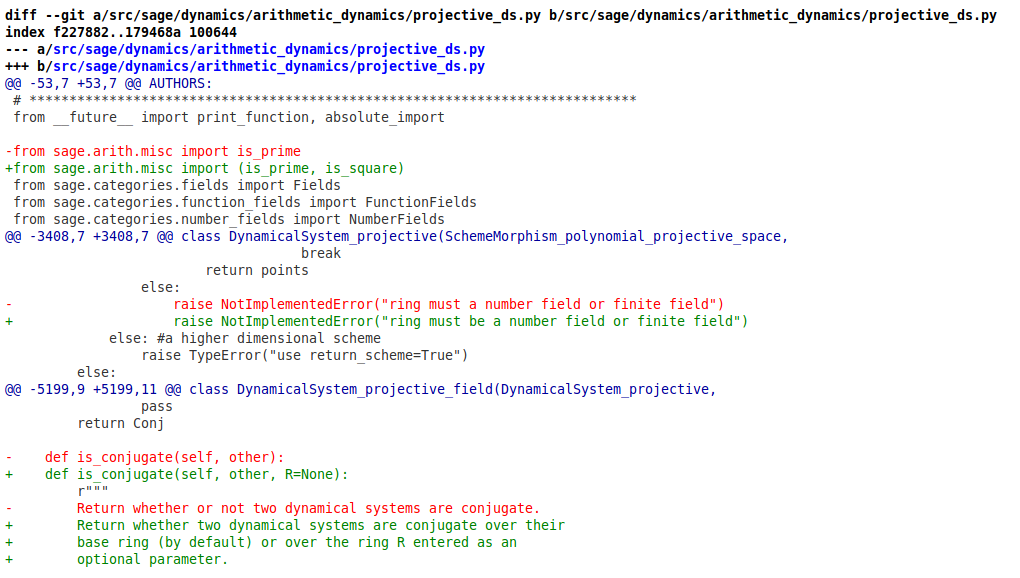
\includegraphics[width=1.1\linewidth]{diff_on_sage_2}}  %ticket 28070
		\only<2>{\item on your files\\
		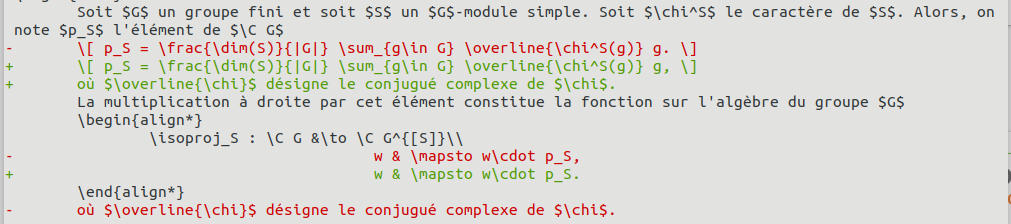
\includegraphics[width=1\linewidth]{diff_on_latex}}
	\end{itemize}
	\end{frame}

	\begin{frame}[fragile]{Reviewing changes\hfill \cmd{diff}}
	To know what has been change since last commit:
	\begin{verbatim}
	$ git diff
	\end{verbatim}
	or since commit1 
	\begin{verbatim}
	$ git diff commit1
	\end{verbatim}
	or between commit1 and commit2
	\begin{verbatim}
	$ git diff commit1 commit2
	\end{verbatim}
	\begin{tcolorbox}[colback=cyan!30]
	To recover the "name" of commit1, you must type \texttt{git log} (this is the history of the repository). The name is very long!\\
	(e.g.: df14e25763073c18e30ebeede3d34ef466dd08c8)
	\end{tcolorbox}
	\end{frame}

	\begin{frame}{Reviewing changes\hfill \cmd{diff}}
	You can do it with a graphical user interface (e.g. Meld 
\includegraphics[height=1em]{meld_logo}).\\
	\vspace{1em}
	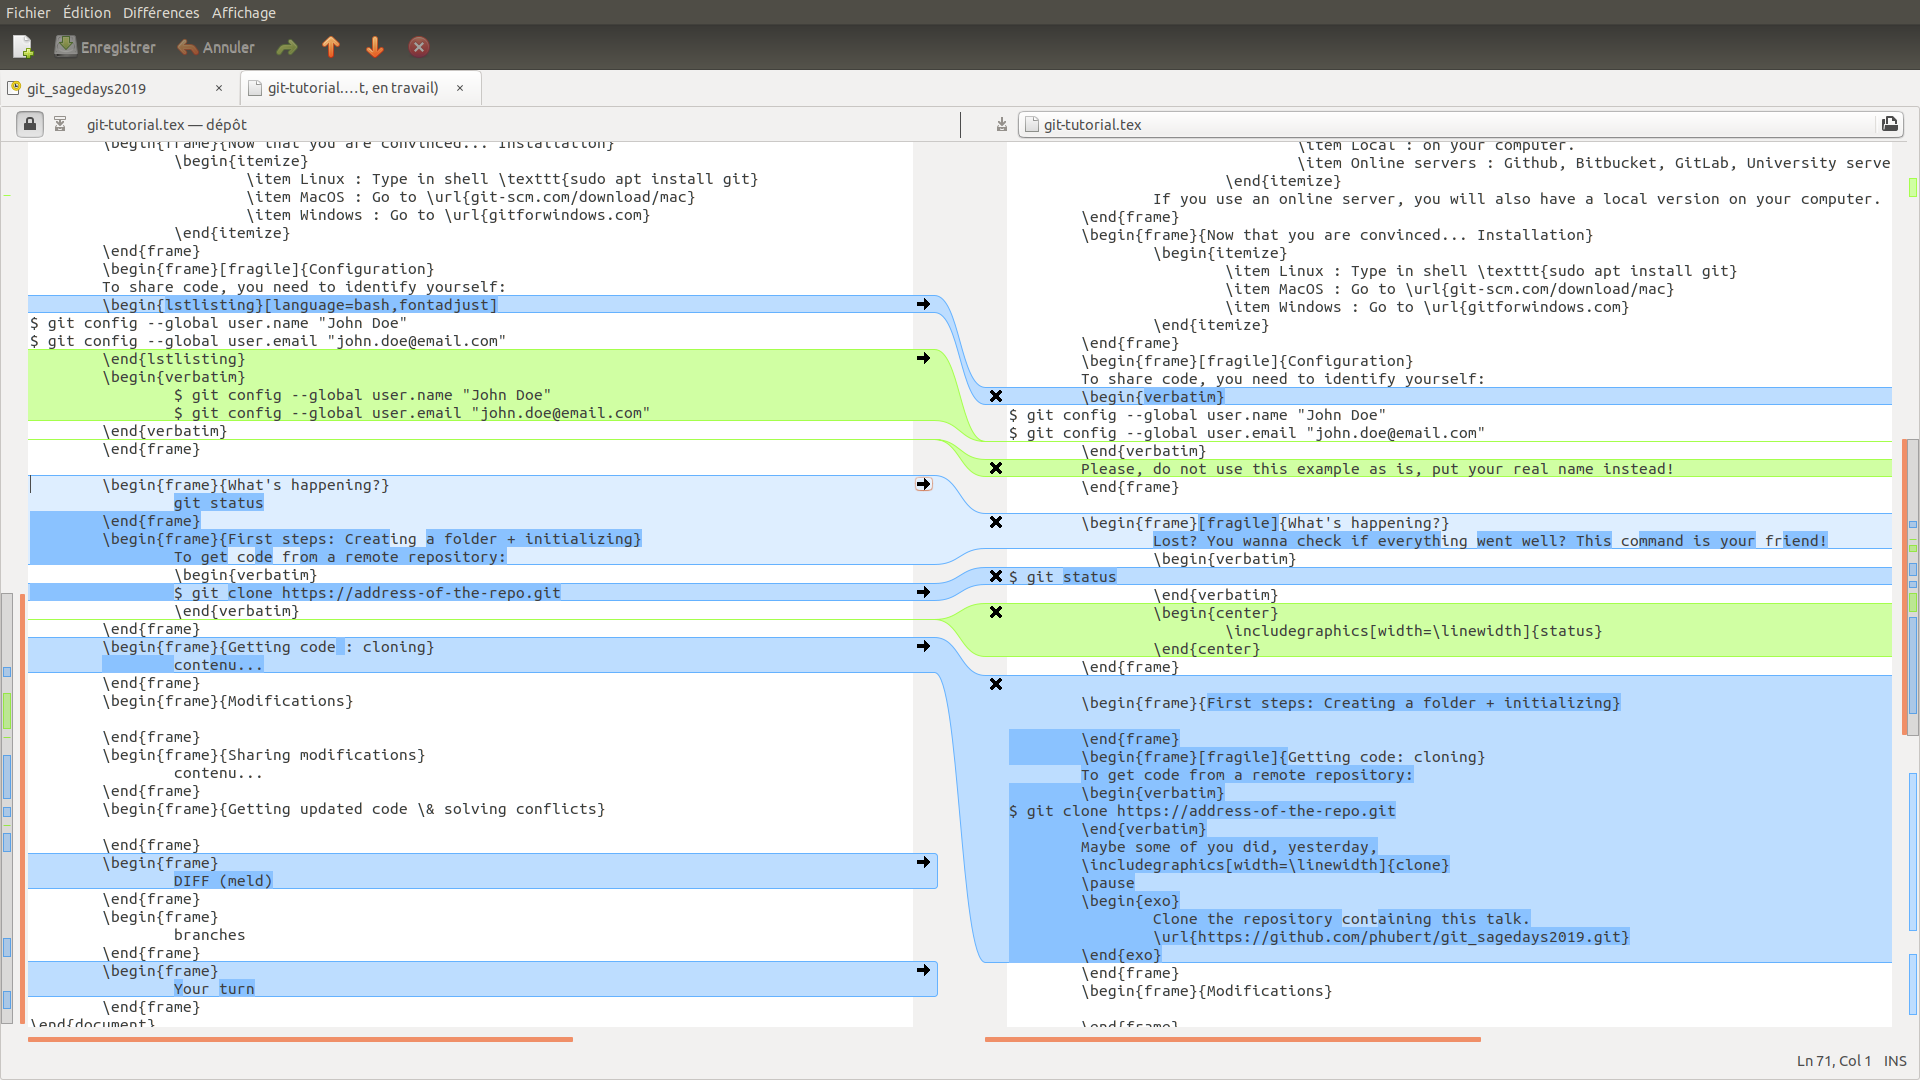
\includegraphics[width=\linewidth]{meld_ps}
	\end{frame}

	\begin{frame}[fragile]{Branches}
		\footnotesize{Image from Bitbucket web site} \vspace{-.5cm}
		\begin{figure}[h]
			\centering
			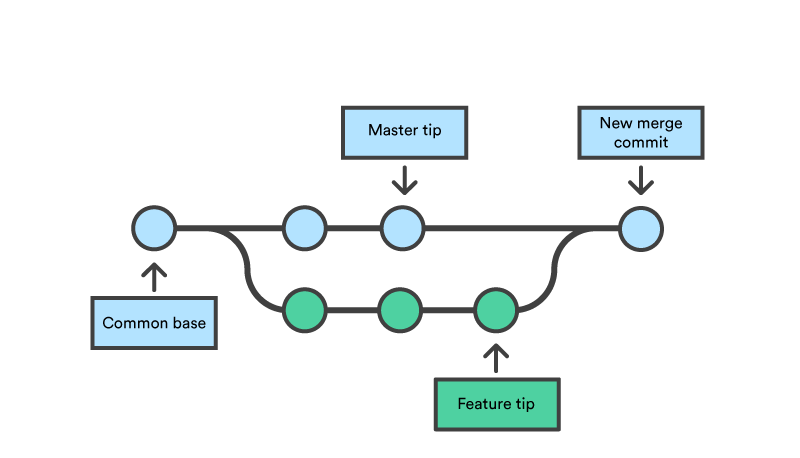
\includegraphics[scale=.3]{branch.png}
		\end{figure}
		
		Create a new branch : \texttt{\$ git branch BRANCH\_NAME}
		
		Navigate between branches : \texttt{\$ git checkout BRANCH\_NAME}
		
		Merge branches : \texttt{\$ git merge BRANCH\_NAME}
	\end{frame}

	\begin{frame}{Conclusion/Moral}
	PLEASE, PLEASE, PLEASE! Read the error messages and outputs.\\
	\vspace{1em}
	\pause
	{\Large Some references}
	\begin{thebibliography}{99}
		\bibitem{SWcarpentry} An awesome tutorial:\\ \url{swcarpentry.github.io/git-novice/}
		\bibitem{tutos} More tutorials, by \href{https://guides.github.com/introduction/git-handbook/}{Github} and \href{https://www.atlassian.com/git/tutorials/learn-git-with-bitbucket-cloud}{BitBucket}
		\bibitem{cheatsheets} Some cheatsheets, by  \href{swcarpentry.github.io/git-novice/reference.html}{Software Carpentry} and \href{https://github.github.com/training-kit/downloads/github-git-cheat-sheet.pdf}{Github}
		\bibitem{servers} Bitbucket, Github and Gitlab all have extended documentation on their website
	\end{thebibliography}
	\end{frame}

	\begin{frame}{Your turn!}
	Two-by-two, try the following:
		\begin{itemize}
			\item Go to the Exercise folder of our repository (you \textit{need} to clone the repository from \url{https://github.com/phubert/git_sagedays2019.git} ).
			\item Create your own branch (name it after the concatenation of your names).
			\item Edit three of the files.
			\item Send your files to the server. \textit{Don't forget to put a relevant commit message!}
			\item We will add mistakes in your files.
			\item Get the modifications and correct the mistakes. Send everything back to us (not by email, of course...)
		\end{itemize}
	\end{frame}


\end{document}
